\section{Kalman-Filter}
Der Kalman-Filter kann verwendet werden, um Iterativ Parameter von Systemzuständen zu schätzen auf der Basis von fehlerbehafteten Beobachtungen und der berechneten physikalischen Formeln. Sie auch \textbf{Beispiel} im Kapitel \ref{kalman}

Der Zustandvektor $x_k$ besteht aus allen Grössen, welche gemessen werden. zB können Position $x(x)$, Geschwindigkeit $v(t)$ und Beschleunigung $a(t)$ gemessen werden. Nach einem Zeitintervall $\Delta t$ kann der neue Zustandsvektor $p_{k+1}$ berechnet werden. Das bedeutet, dass der Neuezustand, anhand der Zeitmatrix $\varphi$ berechnet werden kann: $x_{k+1} = \varphi_kx_k$. Durch sehr kleine $\Delta t$, kann jedes System linearisiert werden.
\[
x_{k+1} = \underbrace{\begin{pmatrix}
	1 & \Delta t & \frac{1}{2}\Delta t^2 \\
	0 & 1 & \Delta t \\
	0 & 0 & 1
\end{pmatrix}}_{\varphi_k}\underbrace{\begin{pmatrix}
x(t) \\ v(t) \\ a(t)
\end{pmatrix}}_{x_k}
\]

Um Messwerte von dem Zustandsvektor $x_k$ herauszulesen, wird eine Hilfsmatrix $H$ eingeführt. Diese soll entscheiden, welcher Sensor welche Messwerte liefert aka Messmatrix $z_k$. Mit folgendem $H$, sind Sensor 1 ein Höhenmesser und Sensor 2 ein Akzelerometer.
\[
 z_k = \underbrace{\begin{pmatrix} 	1 & 0 & 0 \\ 0 & 0 & 1 \end{pmatrix}}_{H_k} \underbrace{\begin{pmatrix}
 		x(t) \\ v(t) \\ a(t)
 \end{pmatrix}}_{x_k}
\]

Um Fehler zu minimieren, müssen Systemfehler $u_k$ (ein Systemmodell welches nicht exakt ist) und Messfehler $w_k$ (Sensoren sind nicht perfekt) berücksichtigt werden. Unter der Annahme, dass Erwartungswerte $E(u_k) = E(w_k) = 0$ sind (keine Systematischen Fehler, welche kompensiert werden könnten) können all diese Fehler mit einer Kovarianz-Matrix $Q$ bzw $R$ zusammengefasst werden. 
\begin{align*}
	Q_k &= E(u_ku^t_k) = \begin{pmatrix}
		\sigma_1^2 & \dots  & 0 \\
		\vdots & \ddots & \vdots \\
		0 & \dots & \sigma^2_n
	\end{pmatrix} \\
	R_k &= E(w_kw^t_k) = \begin{pmatrix}
	\varrho_1^2 & \dots  & 0 \\
	\vdots & \ddots & \vdots \\
	0 & \dots & \varrho^2_m
\end{pmatrix} 
\end{align*}
Um die Schätzfehlerfortpflanzung $f_k$ zu berücksichtigen, werden diese zum Zustandsvektor $x_{k+1}$ addiert $\hat{x}_{k+1} = x_{k+1} \underbrace{- u_k + \varphi_kx_k}_{f_k}$. Dies ergibt die Schätzungsmatrix $P$:
\[
	P_{k+1} = Q_k + \varphi_kP_k\varphi_k^t
\]
Zudem sind Messfehler $g_k$ der Sensoren zu berechnen durch die Messmatrix $z_k$ und dem geschätzten Wert $H_k\hat{x}_k$
\[
G_k = R_k + H_kP_kH^t_k
\]


Eine Schätzung $\hat{x}_{k+1}$ für den neuen Systemzustand kann durch einen Korrekturfaktor von den tatsächlichen Messwerten und den Vorhergesagten Messwerten berechnet werden. Dieser Faktor $K$, auch bekannt als Kalman-Gain ergibt den Kalman-Filter:
\[
\hat{x}_{k+1} = x_{k} + K_k(z_k - H_kx_k)
\] 
$K$ soll nun Optimiert werden, sodas der Schätzfehler bzw. die Varianz minimal wird. 
\[
K_k = P_kH_k^t(H_kP_kH^t_k + R_k)^{-1}
\]
\begin{center}
	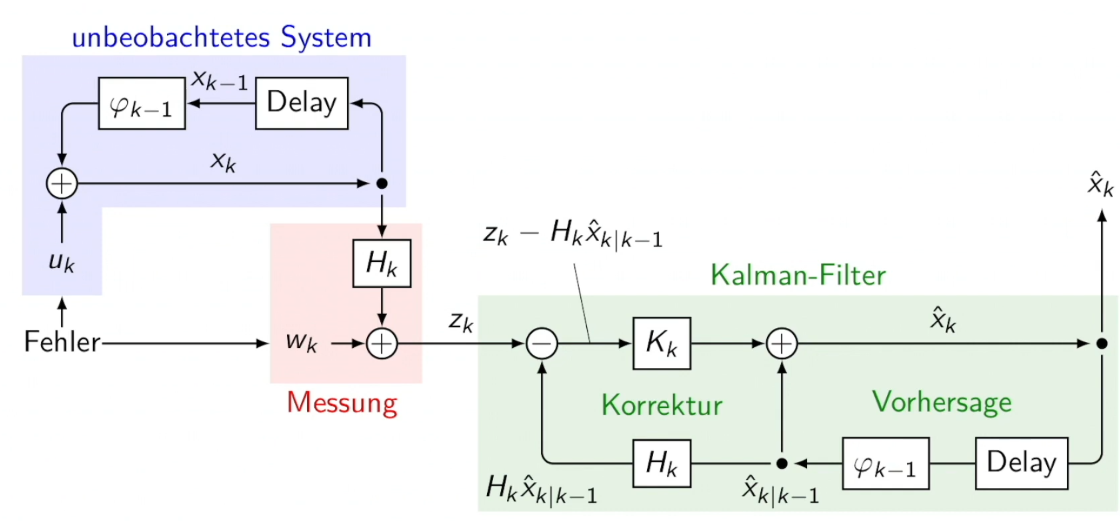
\includegraphics[width=0.9\columnwidth]{Images/kalman}
\end{center}